% !Mode:: "TeX:UTF-8"
% \textbf{计算专题------实数混合运算}

\begin{defproblem}{T16-A04-01}%
\begin{onlyproblem}%
(1)计算:$(\pi -\sqrt 3 )^0+\sqrt {18} -2\sin 45^{\circ}-\left(\dfrac{1}{8}\right)^{-1}+\sqrt[3]{27}$.

\renewcommand{\arraystretch}{1.38}
(2)解方程组:$\left\{\begin{array}{@{}l}
 \dfrac{3x+y}{2}=5 \\ 
 \dfrac{2x-y}{5}=1 \\ 
 \end{array}\right.$.
\end{onlyproblem}%
\begin{onlysolution}%
\begin{center}
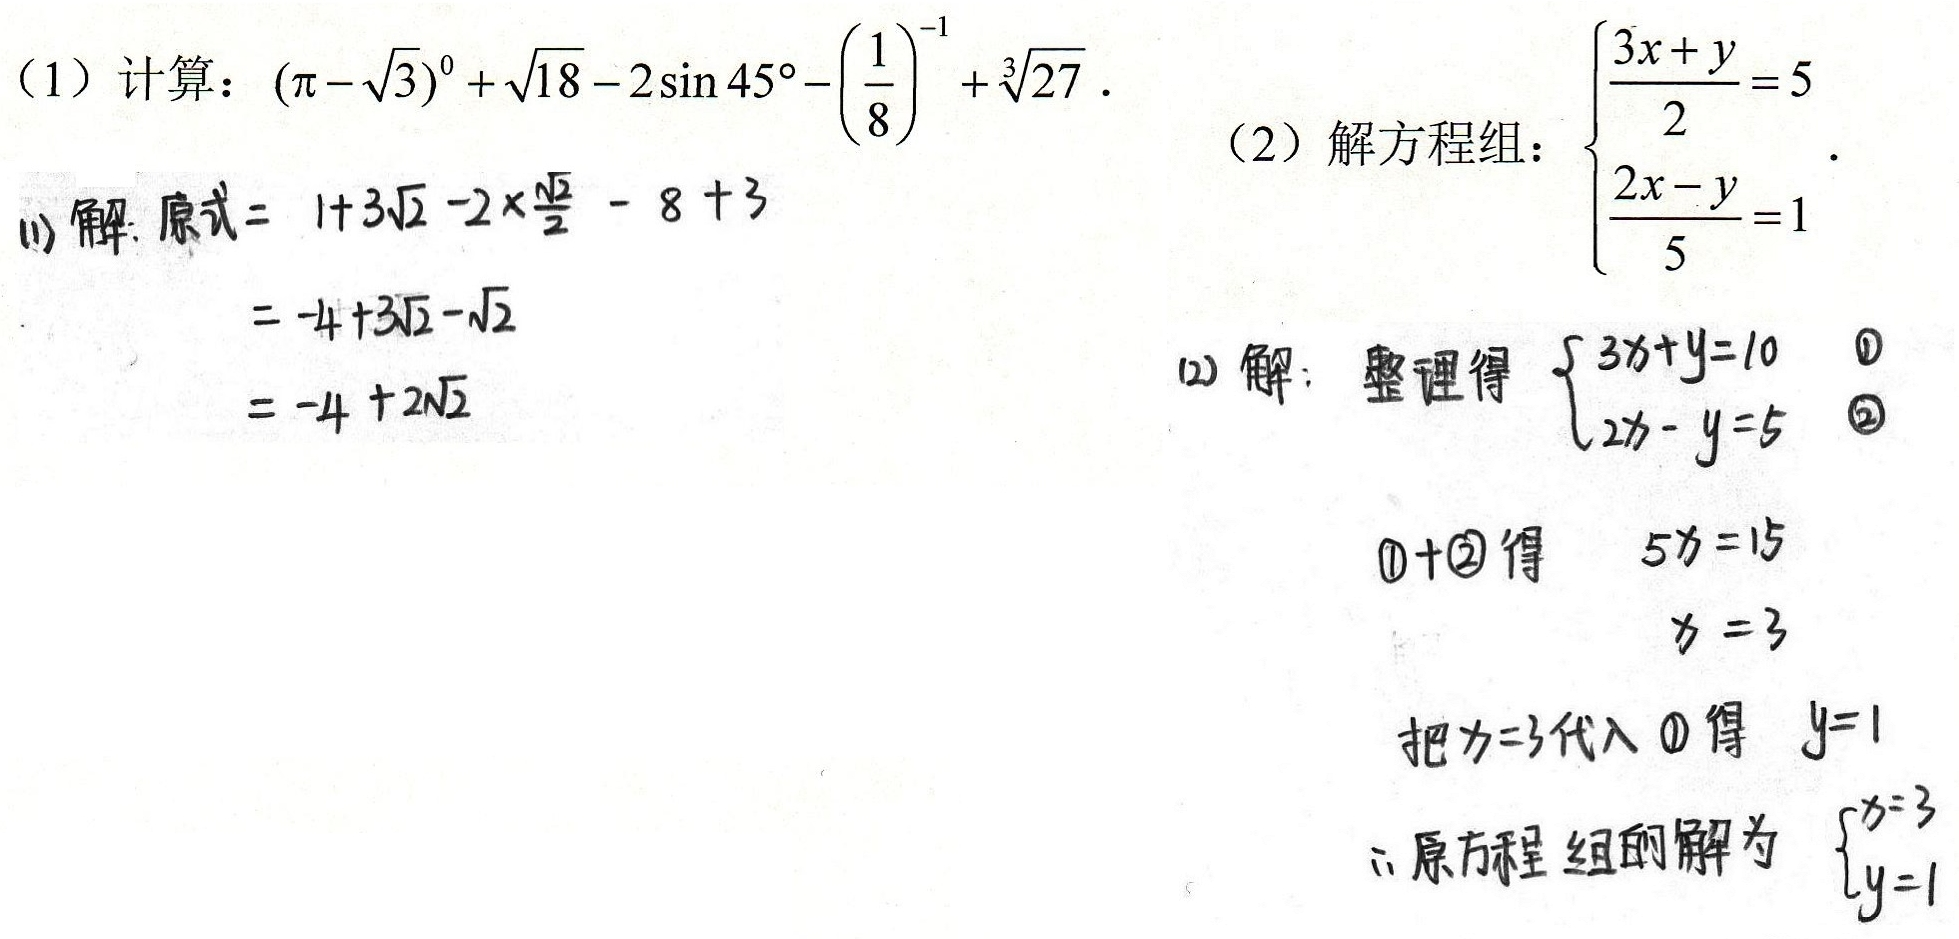
\includegraphics[scale=0.8]{T16-A04-01.jpg}
\end{center}
\end{onlysolution}%
\end{defproblem}


\begin{defproblem}{T16-A04-02}%
\begin{onlyproblem}%

(1)解不等式:$\dfrac{2x-1}{3}-\dfrac{9x-2}{6}\le 1$,并把解集表示在数轴上.


(2)已知关于$x$,$y$的方程组$\left\{\begin{array}{@{}l}
 5x+2y=11a+18 \\ 
 2x-3y=12a-8 \\ 
 \end{array}\right.$的解满足$x>0$,$y>0$,求实数$a$的取值范围.

\end{onlyproblem}%
\begin{onlysolution}%
\begin{center}
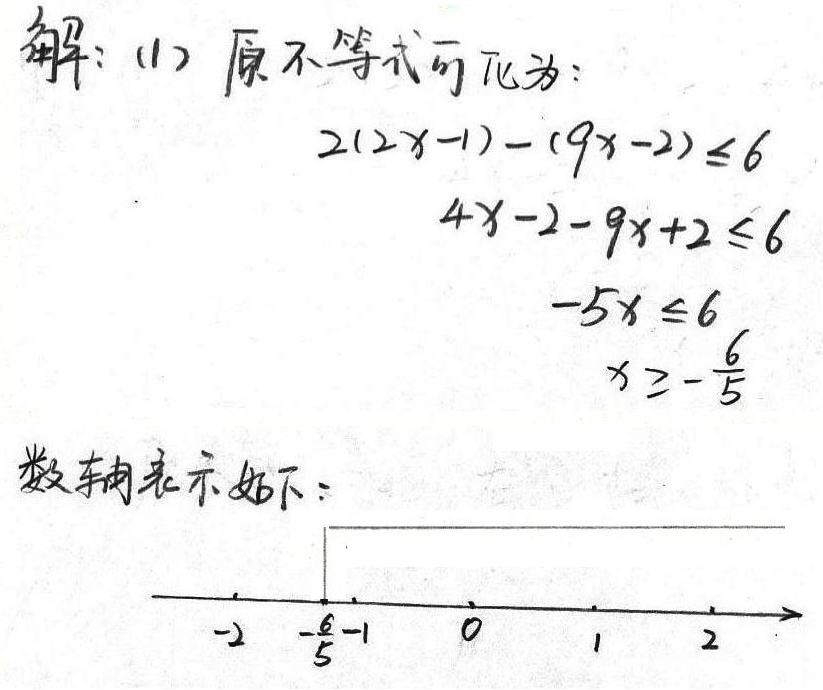
\includegraphics[scale=0.9]{T16-A04-02-1.jpg}
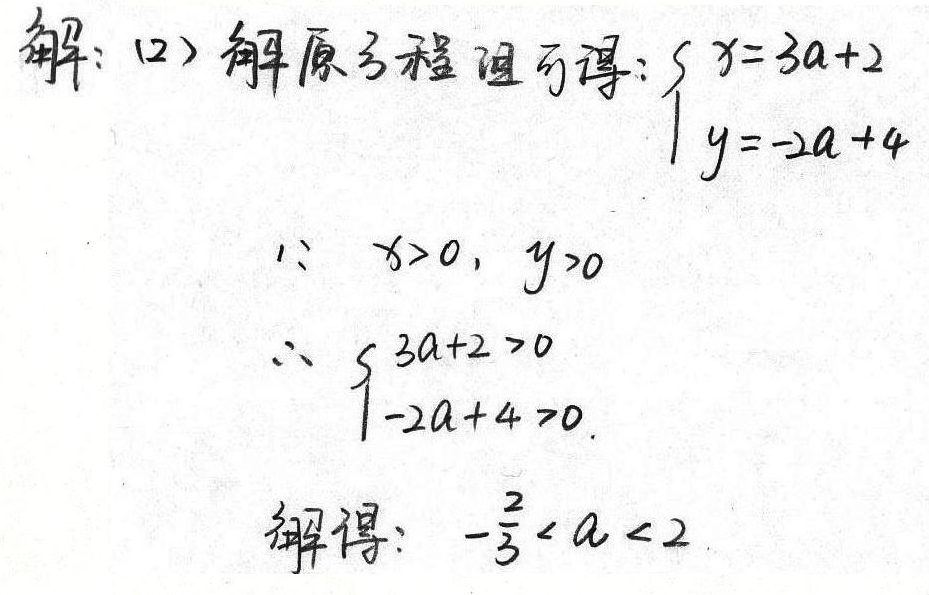
\includegraphics[scale=0.9]{T16-A04-02-2.jpg}
\end{center}
\end{onlysolution}%
\end{defproblem}


\begin{defproblem}{T16-A04-03}%
\begin{onlyproblem}%
(1)计算:$(\sqrt 3 +1)^0+\vert -2\vert -3^{-1}$;


(2)解不等式组:$\left\{\begin{array}{@{}l}
 2x+1<x+5 \\ 
 4x>3x+2 \\ 
 \end{array}\right.$.
\end{onlyproblem}%
\begin{onlysolution}%
\begin{center}
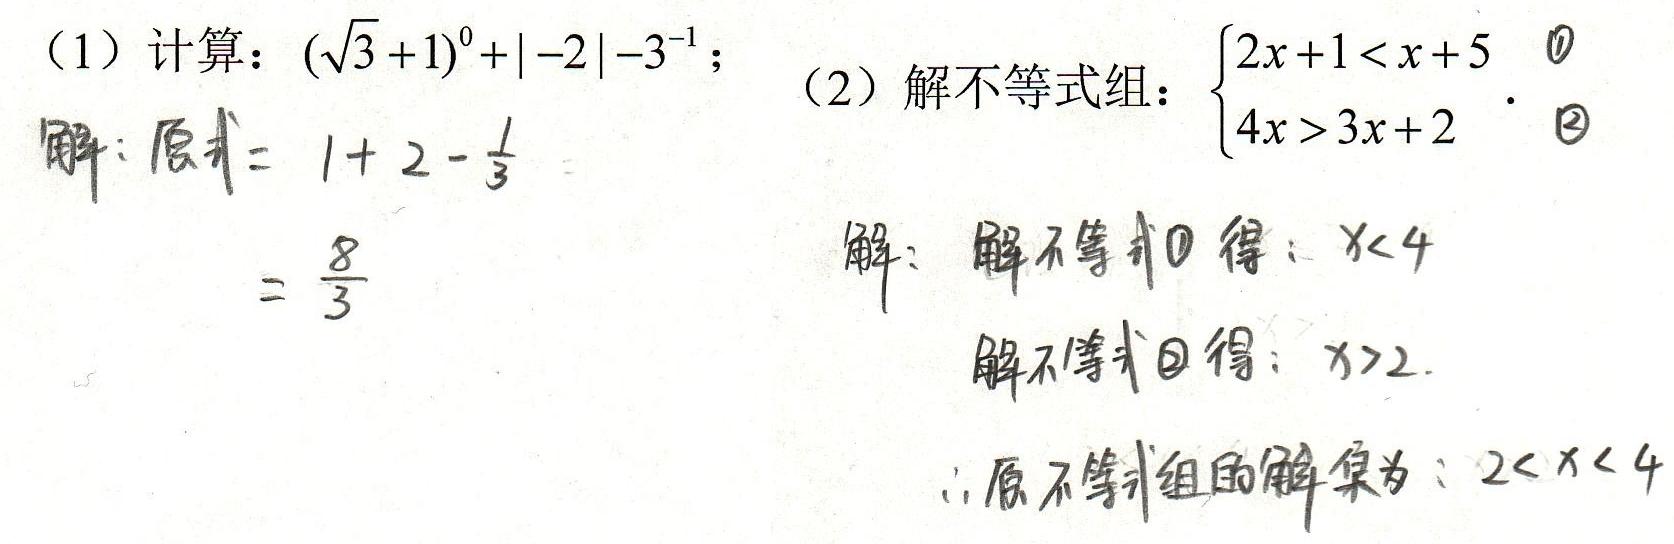
\includegraphics[scale=0.8]{T16-A04-03.jpg}
\end{center}
\end{onlysolution}%
\end{defproblem}


\begin{defproblem}{T16-A04-04}%
\begin{onlyproblem}%

(1)计算:$(\sqrt 2 -3)^0+\left(-\dfrac{1}{2}\right)^{-2}-\vert -2\vert -2\cos 60^{\circ}$;


(2)解方程:$2x^{2}-4x-1=0$.
\end{onlyproblem}%
\begin{onlysolution}%
\begin{center}
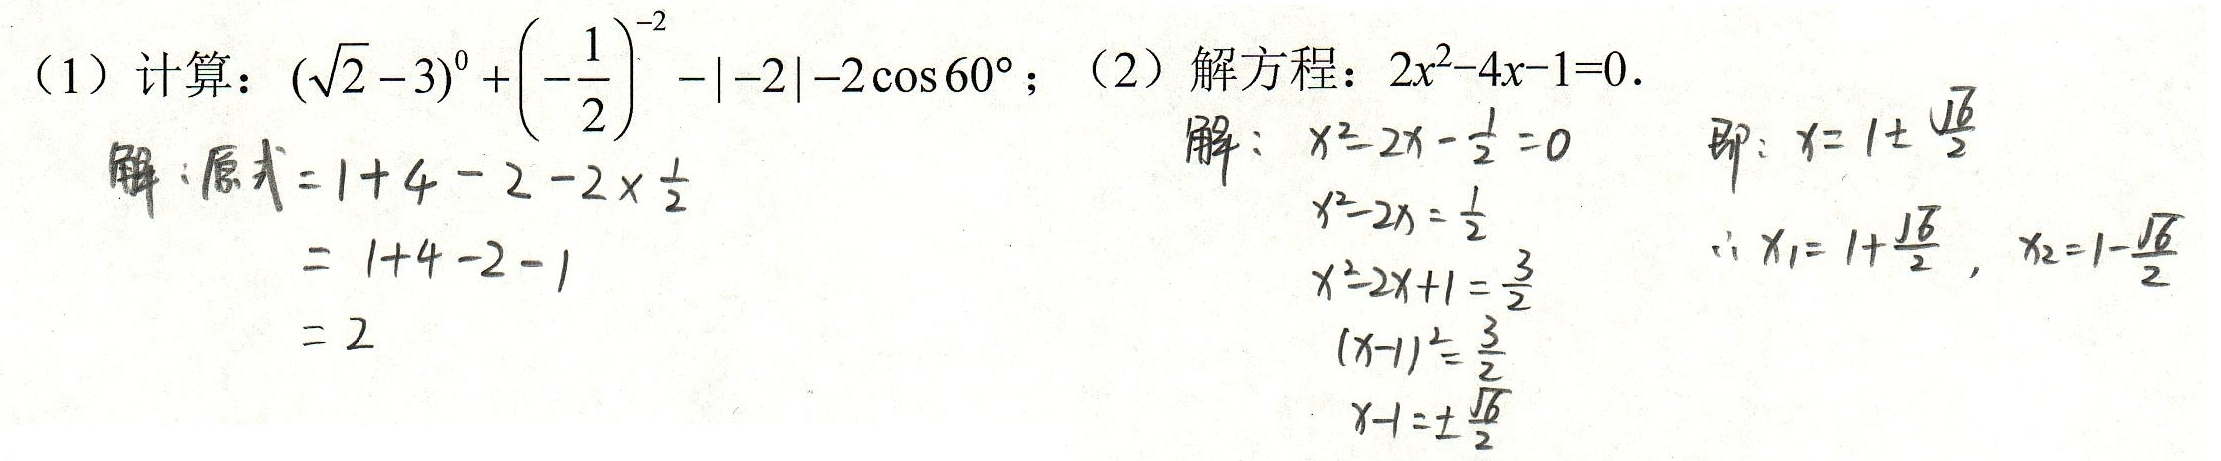
\includegraphics[scale=0.8]{T16-A04-04.jpg}
\end{center}
\end{onlysolution}%
\end{defproblem}


\begin{defproblem}{T16-A04-05}%
\begin{onlyproblem}%
(1)计算:$\sqrt{12}-\sqrt[3]{8}+\vert \sqrt 3 -2\vert $;


(2)化简:$(a+3)(a-2)-a(a-1)$.
\end{onlyproblem}%
\begin{onlysolution}%
\begin{center}
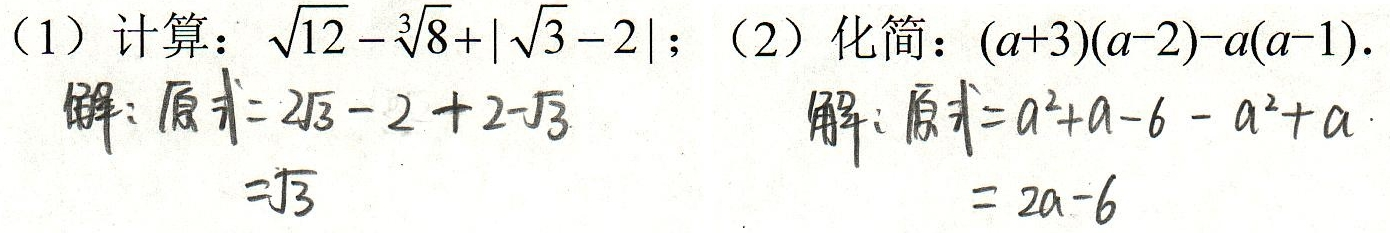
\includegraphics[width=.69\columnwidth]{T16-A04-05.jpg}
\end{center}
\end{onlysolution}%
\end{defproblem}


\begin{defproblem}{T16-A04-06}%
\begin{onlyproblem}%
(1)计算:$(a+1)(a-1)-(a-2)^{2}$;


(2)解不等式:$x-1\ge \dfrac{x-2}{2}+3$.
\end{onlyproblem}%
\begin{onlysolution}%
\begin{center}
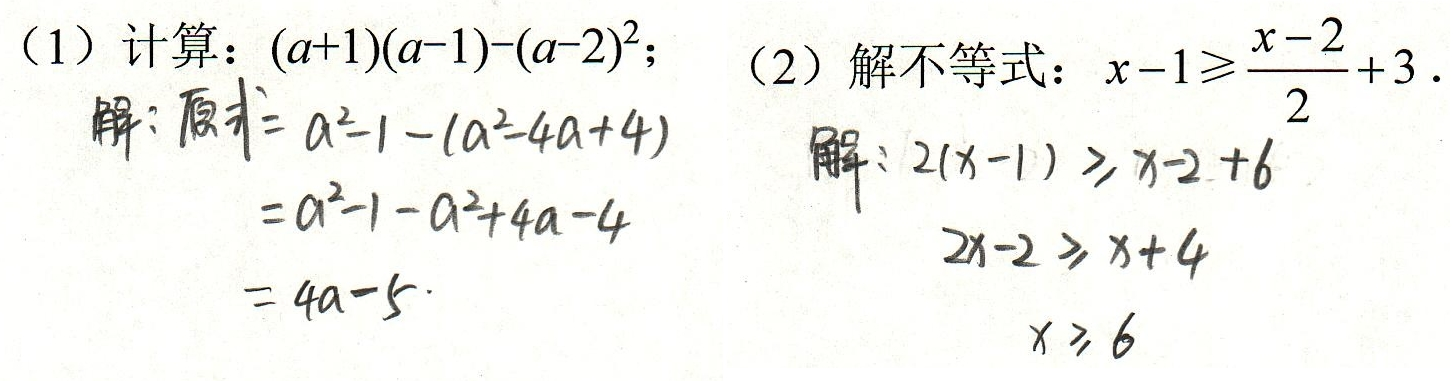
\includegraphics[scale=0.9]{T16-A04-06.jpg}
\end{center}
\end{onlysolution}%
\end{defproblem}

